\documentclass[twoside]{book}

% Packages required by doxygen
\usepackage{fixltx2e}
\usepackage{calc}
\usepackage{doxygen}
\usepackage[export]{adjustbox} % also loads graphicx
\usepackage{graphicx}
\usepackage[utf8]{inputenc}
\usepackage{makeidx}
\usepackage{multicol}
\usepackage{multirow}
\PassOptionsToPackage{warn}{textcomp}
\usepackage{textcomp}
\usepackage[nointegrals]{wasysym}
\usepackage[table]{xcolor}

% Font selection
\usepackage[T1]{fontenc}
\usepackage[scaled=.90]{helvet}
\usepackage{courier}
\usepackage{amssymb}
\usepackage{sectsty}
\renewcommand{\familydefault}{\sfdefault}
\allsectionsfont{%
  \fontseries{bc}\selectfont%
  \color{darkgray}%
}
\renewcommand{\DoxyLabelFont}{%
  \fontseries{bc}\selectfont%
  \color{darkgray}%
}
\newcommand{\+}{\discretionary{\mbox{\scriptsize$\hookleftarrow$}}{}{}}

% Page & text layout
\usepackage{geometry}
\geometry{%
  a4paper,%
  top=2.5cm,%
  bottom=2.5cm,%
  left=2.5cm,%
  right=2.5cm%
}
\tolerance=750
\hfuzz=15pt
\hbadness=750
\setlength{\emergencystretch}{15pt}
\setlength{\parindent}{0cm}
\setlength{\parskip}{3ex plus 2ex minus 2ex}
\makeatletter
\renewcommand{\paragraph}{%
  \@startsection{paragraph}{4}{0ex}{-1.0ex}{1.0ex}{%
    \normalfont\normalsize\bfseries\SS@parafont%
  }%
}
\renewcommand{\subparagraph}{%
  \@startsection{subparagraph}{5}{0ex}{-1.0ex}{1.0ex}{%
    \normalfont\normalsize\bfseries\SS@subparafont%
  }%
}
\makeatother

% Headers & footers
\usepackage{fancyhdr}
\pagestyle{fancyplain}
\fancyhead[LE]{\fancyplain{}{\bfseries\thepage}}
\fancyhead[CE]{\fancyplain{}{}}
\fancyhead[RE]{\fancyplain{}{\bfseries\leftmark}}
\fancyhead[LO]{\fancyplain{}{\bfseries\rightmark}}
\fancyhead[CO]{\fancyplain{}{}}
\fancyhead[RO]{\fancyplain{}{\bfseries\thepage}}
\fancyfoot[LE]{\fancyplain{}{}}
\fancyfoot[CE]{\fancyplain{}{}}
\fancyfoot[RE]{\fancyplain{}{\bfseries\scriptsize Generated by Doxygen }}
\fancyfoot[LO]{\fancyplain{}{\bfseries\scriptsize Generated by Doxygen }}
\fancyfoot[CO]{\fancyplain{}{}}
\fancyfoot[RO]{\fancyplain{}{}}
\renewcommand{\footrulewidth}{0.4pt}
\renewcommand{\chaptermark}[1]{%
  \markboth{#1}{}%
}
\renewcommand{\sectionmark}[1]{%
  \markright{\thesection\ #1}%
}

% Indices & bibliography
\usepackage{natbib}
\usepackage[titles]{tocloft}
\setcounter{tocdepth}{3}
\setcounter{secnumdepth}{5}
\makeindex

% Hyperlinks (required, but should be loaded last)
\usepackage{ifpdf}
\ifpdf
  \usepackage[pdftex,pagebackref=true]{hyperref}
\else
  \usepackage[ps2pdf,pagebackref=true]{hyperref}
\fi
\hypersetup{%
  colorlinks=true,%
  linkcolor=blue,%
  citecolor=blue,%
  unicode%
}

% Custom commands
\newcommand{\clearemptydoublepage}{%
  \newpage{\pagestyle{empty}\cleardoublepage}%
}

\usepackage{caption}
\captionsetup{labelsep=space,justification=centering,font={bf},singlelinecheck=off,skip=4pt,position=top}

%===== C O N T E N T S =====

\begin{document}

% Titlepage & ToC
\hypersetup{pageanchor=false,
             bookmarksnumbered=true,
             pdfencoding=unicode
            }
\pagenumbering{alph}
\begin{titlepage}
\vspace*{7cm}
\begin{center}%
{\Large T\+T\+K4235\+: Elevator project }\\
\vspace*{1cm}
{\large Generated by Doxygen 1.8.13}\\
\end{center}
\end{titlepage}
\clearemptydoublepage
\pagenumbering{roman}
\tableofcontents
\clearemptydoublepage
\pagenumbering{arabic}
\hypersetup{pageanchor=true}

%--- Begin generated contents ---
\chapter{Data Structure Index}
\section{Data Structures}
Here are the data structures with brief descriptions\+:\begin{DoxyCompactList}
\item\contentsline{section}{\hyperlink{structFSMPosition}{F\+S\+M\+Position} \\*Elevator position used in {\ttfamily \hyperlink{fsm_8c_source}{fsm.\+c}} }{\pageref{structFSMPosition}}{}
\end{DoxyCompactList}

\chapter{File Index}
\section{File List}
Here is a list of all documented files with brief descriptions\+:\begin{DoxyCompactList}
\item\contentsline{section}{source/{\bfseries example.\+c} }{\pageref{example_8c}}{}
\item\contentsline{section}{source/{\bfseries fsm.\+c} }{\pageref{fsm_8c}}{}
\item\contentsline{section}{source/\hyperlink{fsm_8h}{fsm.\+h} \\*Functions to handle events in finite state machine, based on current state }{\pageref{fsm_8h}}{}
\item\contentsline{section}{source/\hyperlink{fsm__types_8h}{fsm\+\_\+types.\+h} \\*Struct and enums for the finite state machine }{\pageref{fsm__types_8h}}{}
\item\contentsline{section}{source/\hyperlink{hardware_8h}{hardware.\+h} \\*Driver for the elevator hardware }{\pageref{hardware_8h}}{}
\item\contentsline{section}{source/{\bfseries main.\+c} }{\pageref{main_8c}}{}
\item\contentsline{section}{source/{\bfseries orders.\+c} }{\pageref{orders_8c}}{}
\item\contentsline{section}{source/\hyperlink{orders_8h}{orders.\+h} \\*Functions to collect, prioritize and delete orders }{\pageref{orders_8h}}{}
\item\contentsline{section}{source/{\bfseries timer.\+c} }{\pageref{timer_8c}}{}
\item\contentsline{section}{source/\hyperlink{timer_8h}{timer.\+h} \\*Functions to stop and start timer, and detect a timeout }{\pageref{timer_8h}}{}
\end{DoxyCompactList}

\chapter{Data Structure Documentation}
\hypertarget{structFSMPosition}{}\section{F\+S\+M\+Position Struct Reference}
\label{structFSMPosition}\index{F\+S\+M\+Position@{F\+S\+M\+Position}}


Elevator position used in {\ttfamily \hyperlink{fsm_8c_source}{fsm.\+c}}.  




{\ttfamily \#include $<$fsm\+\_\+types.\+h$>$}

\subsection*{Data Fields}
\begin{DoxyCompactItemize}
\item 
\mbox{\Hypertarget{structFSMPosition_a40c73f44ee3cb7ca8062f71d2001ecf2}\label{structFSMPosition_a40c73f44ee3cb7ca8062f71d2001ecf2}} 
int {\bfseries floor}
\item 
\mbox{\Hypertarget{structFSMPosition_a7f8cfe43199b380c6621f1f932a7e75a}\label{structFSMPosition_a7f8cfe43199b380c6621f1f932a7e75a}} 
int {\bfseries above}
\end{DoxyCompactItemize}


\subsection{Detailed Description}
Elevator position used in {\ttfamily \hyperlink{fsm_8c_source}{fsm.\+c}}. 

Definition at line 23 of file fsm\+\_\+types.\+h.



The documentation for this struct was generated from the following file\+:\begin{DoxyCompactItemize}
\item 
source/\hyperlink{fsm__types_8h}{fsm\+\_\+types.\+h}\end{DoxyCompactItemize}

\chapter{File Documentation}
\hypertarget{fsm_8h}{}\section{source/fsm.h File Reference}
\label{fsm_8h}\index{source/fsm.\+h@{source/fsm.\+h}}


Functions to handle events in finite state machine, based on current state.  


{\ttfamily \#include \char`\"{}hardware.\+h\char`\"{}}\newline
{\ttfamily \#include \char`\"{}orders.\+h\char`\"{}}\newline
{\ttfamily \#include \char`\"{}fsm\+\_\+types.\+h\char`\"{}}\newline
{\ttfamily \#include \char`\"{}timer.\+h\char`\"{}}\newline
Include dependency graph for fsm.\+h\+:
\nopagebreak
\begin{figure}[H]
\begin{center}
\leavevmode
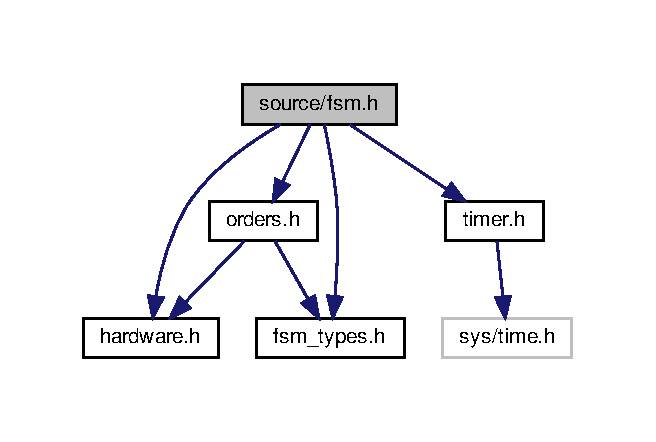
\includegraphics[width=315pt]{fsm_8h__incl}
\end{center}
\end{figure}
This graph shows which files directly or indirectly include this file\+:
\nopagebreak
\begin{figure}[H]
\begin{center}
\leavevmode
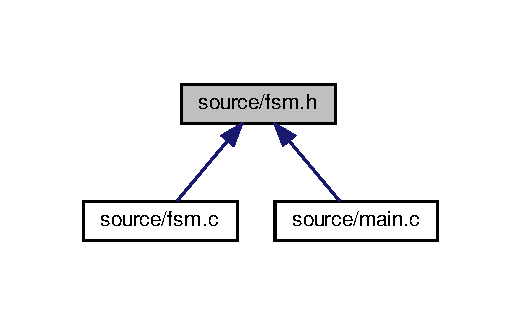
\includegraphics[width=250pt]{fsm_8h__dep__incl}
\end{center}
\end{figure}
\subsection*{Functions}
\begin{DoxyCompactItemize}
\item 
\mbox{\Hypertarget{fsm_8h_a1a4806578fc4f6c172850f81d64c63c1}\label{fsm_8h_a1a4806578fc4f6c172850f81d64c63c1}} 
void \hyperlink{fsm_8h_a1a4806578fc4f6c172850f81d64c63c1}{fsm\+\_\+initialize} ()
\begin{DoxyCompactList}\small\item\em Initialize elevator and change state to {\ttfamily F\+S\+M\+\_\+\+Initialize}. \end{DoxyCompactList}\item 
void \hyperlink{fsm_8h_a684459231edf4861a2ef1b2ec1c9edd4}{fsm\+\_\+floor\+\_\+reached} (int floor)
\begin{DoxyCompactList}\small\item\em A {\ttfamily floor} has been reached. Update current floor and check if state should be changed. \end{DoxyCompactList}\item 
void \hyperlink{fsm_8h_aea668ded2e4538d10632abf7c30d220c}{fsm\+\_\+new\+\_\+order} (int floor, \hyperlink{hardware_8h_a796a8de8ce0ae769d7dbd3327a7bdbe7}{Hardware\+Order} order\+\_\+type)
\begin{DoxyCompactList}\small\item\em A new order at {\ttfamily floor} of type {\ttfamily order\+\_\+type} has been registered. Check if order should be handled and if state should be changed. \end{DoxyCompactList}\item 
\mbox{\Hypertarget{fsm_8h_a87b2316f536dd22d0fff88d73cfe90b7}\label{fsm_8h_a87b2316f536dd22d0fff88d73cfe90b7}} 
void \hyperlink{fsm_8h_a87b2316f536dd22d0fff88d73cfe90b7}{fsm\+\_\+timeout} ()
\begin{DoxyCompactList}\small\item\em The timer has timed out. If current state is {\ttfamily F\+S\+M\+\_\+\+O\+P\+EN}, close door and change state. \end{DoxyCompactList}\item 
\mbox{\Hypertarget{fsm_8h_a9e75ce9afc9bbf043603abb191769f2e}\label{fsm_8h_a9e75ce9afc9bbf043603abb191769f2e}} 
void \hyperlink{fsm_8h_a9e75ce9afc9bbf043603abb191769f2e}{fsm\+\_\+obstruction\+\_\+detected} ()
\begin{DoxyCompactList}\small\item\em An obstruction has been detected. If current state is {\ttfamily F\+S\+M\+\_\+\+O\+P\+EN}, keep door open. \end{DoxyCompactList}\item 
\mbox{\Hypertarget{fsm_8h_affbbc74a5f9e1e4720c4be1853aeb3d3}\label{fsm_8h_affbbc74a5f9e1e4720c4be1853aeb3d3}} 
void \hyperlink{fsm_8h_affbbc74a5f9e1e4720c4be1853aeb3d3}{fsm\+\_\+stop\+\_\+pressed} ()
\begin{DoxyCompactList}\small\item\em The stop button has been pressed. Stop all motion, delete orders and change state. If elevator is at a floor, open door. \end{DoxyCompactList}\item 
\mbox{\Hypertarget{fsm_8h_a8c53ec8f3b4ba0eac83053852f8076b8}\label{fsm_8h_a8c53ec8f3b4ba0eac83053852f8076b8}} 
void \hyperlink{fsm_8h_a8c53ec8f3b4ba0eac83053852f8076b8}{fsm\+\_\+stop\+\_\+released} ()
\begin{DoxyCompactList}\small\item\em The stop button has been released. If current state is {\ttfamily F\+S\+M\+\_\+\+S\+T\+OP}, change state. \end{DoxyCompactList}\end{DoxyCompactItemize}


\subsection{Detailed Description}
Functions to handle events in finite state machine, based on current state. 



\subsection{Function Documentation}
\mbox{\Hypertarget{fsm_8h_a684459231edf4861a2ef1b2ec1c9edd4}\label{fsm_8h_a684459231edf4861a2ef1b2ec1c9edd4}} 
\index{fsm.\+h@{fsm.\+h}!fsm\+\_\+floor\+\_\+reached@{fsm\+\_\+floor\+\_\+reached}}
\index{fsm\+\_\+floor\+\_\+reached@{fsm\+\_\+floor\+\_\+reached}!fsm.\+h@{fsm.\+h}}
\subsubsection{\texorpdfstring{fsm\+\_\+floor\+\_\+reached()}{fsm\_floor\_reached()}}
{\footnotesize\ttfamily void fsm\+\_\+floor\+\_\+reached (\begin{DoxyParamCaption}\item[{int}]{floor }\end{DoxyParamCaption})}



A {\ttfamily floor} has been reached. Update current floor and check if state should be changed. 


\begin{DoxyParams}[1]{Parameters}
\mbox{\tt in}  & {\em floor} & \\
\hline
\end{DoxyParams}


Definition at line 40 of file fsm.\+c.

\mbox{\Hypertarget{fsm_8h_aea668ded2e4538d10632abf7c30d220c}\label{fsm_8h_aea668ded2e4538d10632abf7c30d220c}} 
\index{fsm.\+h@{fsm.\+h}!fsm\+\_\+new\+\_\+order@{fsm\+\_\+new\+\_\+order}}
\index{fsm\+\_\+new\+\_\+order@{fsm\+\_\+new\+\_\+order}!fsm.\+h@{fsm.\+h}}
\subsubsection{\texorpdfstring{fsm\+\_\+new\+\_\+order()}{fsm\_new\_order()}}
{\footnotesize\ttfamily void fsm\+\_\+new\+\_\+order (\begin{DoxyParamCaption}\item[{int}]{floor,  }\item[{\hyperlink{hardware_8h_a796a8de8ce0ae769d7dbd3327a7bdbe7}{Hardware\+Order}}]{order\+\_\+type }\end{DoxyParamCaption})}



A new order at {\ttfamily floor} of type {\ttfamily order\+\_\+type} has been registered. Check if order should be handled and if state should be changed. 


\begin{DoxyParams}[1]{Parameters}
\mbox{\tt in}  & {\em floor} & \\
\hline
\mbox{\tt in}  & {\em order\+\_\+type} & \\
\hline
\end{DoxyParams}


Definition at line 65 of file fsm.\+c.


\hypertarget{fsm__types_8h}{}\section{source/fsm\+\_\+types.h File Reference}
\label{fsm__types_8h}\index{source/fsm\+\_\+types.\+h@{source/fsm\+\_\+types.\+h}}


Struct and enums for the finite state machine.  


This graph shows which files directly or indirectly include this file\+:
\nopagebreak
\begin{figure}[H]
\begin{center}
\leavevmode
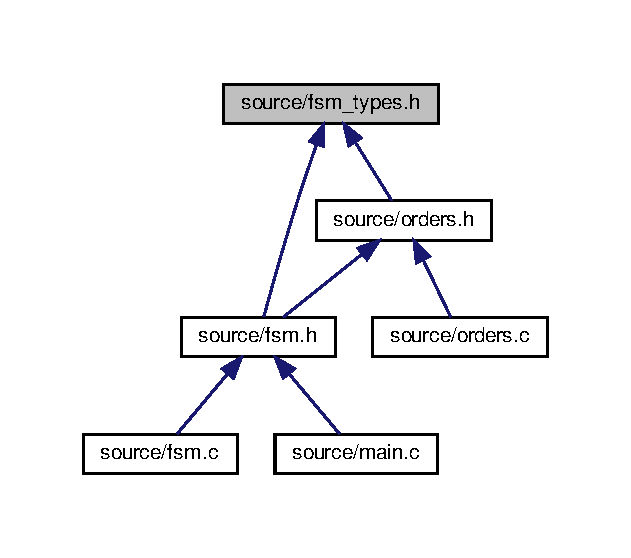
\includegraphics[width=303pt]{fsm__types_8h__dep__incl}
\end{center}
\end{figure}
\subsection*{Data Structures}
\begin{DoxyCompactItemize}
\item 
struct \hyperlink{structFSMPosition}{F\+S\+M\+Position}
\begin{DoxyCompactList}\small\item\em Elevator position used in {\ttfamily \hyperlink{fsm_8c_source}{fsm.\+c}}. \end{DoxyCompactList}\end{DoxyCompactItemize}
\subsection*{Enumerations}
\begin{DoxyCompactItemize}
\item 
\mbox{\Hypertarget{fsm__types_8h_a4a597c1235e9a9b2d218ed5c4c033303}\label{fsm__types_8h_a4a597c1235e9a9b2d218ed5c4c033303}} 
enum \hyperlink{fsm__types_8h_a4a597c1235e9a9b2d218ed5c4c033303}{F\+S\+M\+State} \{ \newline
{\bfseries F\+S\+M\+\_\+\+I\+N\+I\+T\+I\+A\+L\+I\+ZE}, 
{\bfseries F\+S\+M\+\_\+\+I\+D\+LE}, 
{\bfseries F\+S\+M\+\_\+\+M\+O\+V\+I\+NG}, 
{\bfseries F\+S\+M\+\_\+\+O\+P\+EN}, 
\newline
{\bfseries F\+S\+M\+\_\+\+S\+T\+OP}
 \}\begin{DoxyCompactList}\small\item\em Elevator states used in {\ttfamily \hyperlink{fsm_8c_source}{fsm.\+c}}. \end{DoxyCompactList}
\item 
\mbox{\Hypertarget{fsm__types_8h_a5b298403c88d636ded80069711480dae}\label{fsm__types_8h_a5b298403c88d636ded80069711480dae}} 
enum \hyperlink{fsm__types_8h_a5b298403c88d636ded80069711480dae}{F\+S\+M\+Direction} \{ {\bfseries F\+S\+M\+\_\+\+D\+I\+R\+E\+C\+T\+I\+O\+N\+\_\+\+UP}, 
{\bfseries F\+S\+M\+\_\+\+D\+I\+R\+E\+C\+T\+I\+O\+N\+\_\+\+D\+O\+WN}
 \}\begin{DoxyCompactList}\small\item\em Elevator direction used in {\ttfamily \hyperlink{fsm_8c_source}{fsm.\+c}} and {\ttfamily \hyperlink{orders_8c_source}{orders.\+c}}. \end{DoxyCompactList}
\end{DoxyCompactItemize}


\subsection{Detailed Description}
Struct and enums for the finite state machine. 


\hypertarget{hardware_8h}{}\section{source/hardware.h File Reference}
\label{hardware_8h}\index{source/hardware.\+h@{source/hardware.\+h}}


Driver for the elevator hardware.  


This graph shows which files directly or indirectly include this file\+:
\nopagebreak
\begin{figure}[H]
\begin{center}
\leavevmode
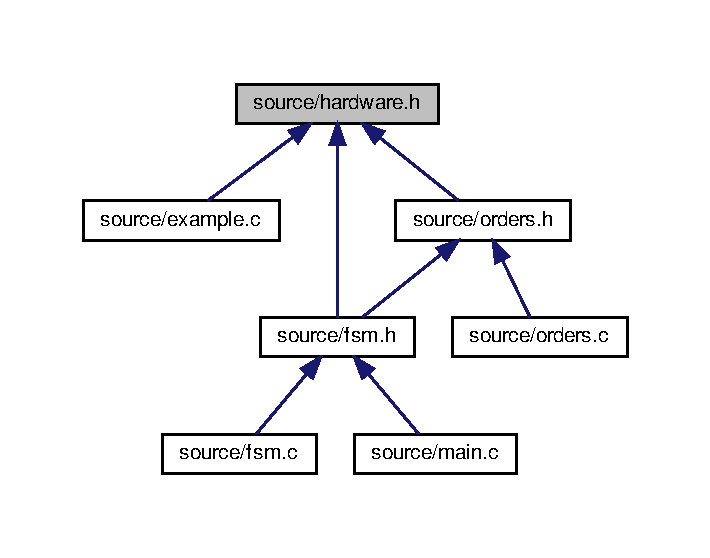
\includegraphics[width=341pt]{hardware_8h__dep__incl}
\end{center}
\end{figure}
\subsection*{Macros}
\begin{DoxyCompactItemize}
\item 
\mbox{\Hypertarget{hardware_8h_ae9e42615eade15633bd8c03b7a271a00}\label{hardware_8h_ae9e42615eade15633bd8c03b7a271a00}} 
\#define {\bfseries H\+A\+R\+D\+W\+A\+R\+E\+\_\+\+N\+U\+M\+B\+E\+R\+\_\+\+O\+F\+\_\+\+F\+L\+O\+O\+RS}~4
\end{DoxyCompactItemize}
\subsection*{Enumerations}
\begin{DoxyCompactItemize}
\item 
\mbox{\Hypertarget{hardware_8h_a2167c399a24df296afc432bcb88228af}\label{hardware_8h_a2167c399a24df296afc432bcb88228af}} 
enum \hyperlink{hardware_8h_a2167c399a24df296afc432bcb88228af}{Hardware\+Movement} \{ {\bfseries H\+A\+R\+D\+W\+A\+R\+E\+\_\+\+M\+O\+V\+E\+M\+E\+N\+T\+\_\+\+UP}, 
{\bfseries H\+A\+R\+D\+W\+A\+R\+E\+\_\+\+M\+O\+V\+E\+M\+E\+N\+T\+\_\+\+S\+T\+OP}, 
{\bfseries H\+A\+R\+D\+W\+A\+R\+E\+\_\+\+M\+O\+V\+E\+M\+E\+N\+T\+\_\+\+D\+O\+WN}
 \}\begin{DoxyCompactList}\small\item\em Movement type used in {\ttfamily hardware\+\_\+command\+\_\+movement}. \end{DoxyCompactList}
\item 
\mbox{\Hypertarget{hardware_8h_a796a8de8ce0ae769d7dbd3327a7bdbe7}\label{hardware_8h_a796a8de8ce0ae769d7dbd3327a7bdbe7}} 
enum \hyperlink{hardware_8h_a796a8de8ce0ae769d7dbd3327a7bdbe7}{Hardware\+Order} \{ {\bfseries H\+A\+R\+D\+W\+A\+R\+E\+\_\+\+O\+R\+D\+E\+R\+\_\+\+UP}, 
{\bfseries H\+A\+R\+D\+W\+A\+R\+E\+\_\+\+O\+R\+D\+E\+R\+\_\+\+I\+N\+S\+I\+DE}, 
{\bfseries H\+A\+R\+D\+W\+A\+R\+E\+\_\+\+O\+R\+D\+E\+R\+\_\+\+D\+O\+WN}
 \}\begin{DoxyCompactList}\small\item\em Order type used in {\ttfamily hardware\+\_\+read\+\_\+order} and in {\ttfamily hardware\+\_\+command\+\_\+order\+\_\+light}. \end{DoxyCompactList}
\end{DoxyCompactItemize}
\subsection*{Functions}
\begin{DoxyCompactItemize}
\item 
int \hyperlink{hardware_8h_a054b8fb8768311d46be58d6a4890d771}{hardware\+\_\+init} ()
\begin{DoxyCompactList}\small\item\em Initializes the elevator control hardware. Must be called once before other calls to the elevator hardware driver. \end{DoxyCompactList}\item 
void \hyperlink{hardware_8h_a01de081ef0510a111053c18cd31afa27}{hardware\+\_\+command\+\_\+movement} (\hyperlink{hardware_8h_a2167c399a24df296afc432bcb88228af}{Hardware\+Movement} movement)
\begin{DoxyCompactList}\small\item\em Commands the elevator to either move up or down, or commands it to halt. \end{DoxyCompactList}\item 
int \hyperlink{hardware_8h_a4a77b27c86675c00b513db3445966804}{hardware\+\_\+read\+\_\+stop\+\_\+signal} ()
\begin{DoxyCompactList}\small\item\em Polls the hardware for the current stop signal. \end{DoxyCompactList}\item 
int \hyperlink{hardware_8h_a459fe57a3ee4bc2a28e8a15b2ab14c2d}{hardware\+\_\+read\+\_\+obstruction\+\_\+signal} ()
\begin{DoxyCompactList}\small\item\em Polls the hardware for the current obstruction signal. \end{DoxyCompactList}\item 
int \hyperlink{hardware_8h_ab048489e6302bb5604aad753f2d7d501}{hardware\+\_\+read\+\_\+floor\+\_\+sensor} (int floor)
\begin{DoxyCompactList}\small\item\em Polls the floor sensor for the given {\ttfamily floor}. \end{DoxyCompactList}\item 
int \hyperlink{hardware_8h_a87917f3aa093fb46ca821a400d011ee8}{hardware\+\_\+read\+\_\+order} (int floor, \hyperlink{hardware_8h_a796a8de8ce0ae769d7dbd3327a7bdbe7}{Hardware\+Order} order\+\_\+type)
\begin{DoxyCompactList}\small\item\em Polls the hardware for the status of orders from floor {\ttfamily floor} of type {\ttfamily order\+\_\+type}. \end{DoxyCompactList}\item 
void \hyperlink{hardware_8h_a80d99ddaa8e7b58c9a88b60ea553c1b6}{hardware\+\_\+command\+\_\+door\+\_\+open} (int door\+\_\+open)
\begin{DoxyCompactList}\small\item\em Commands the hardware to open-\/ or close the elevator door. \end{DoxyCompactList}\item 
void \hyperlink{hardware_8h_a407a6ec035ba357de6aa0fbe55501d1e}{hardware\+\_\+command\+\_\+floor\+\_\+indicator\+\_\+on} (int floor)
\begin{DoxyCompactList}\small\item\em Commands the hardware to turn on the floor indicator for {\ttfamily floor}. All indicators all mutually exclusive; other indicator lights will turn off. \end{DoxyCompactList}\item 
void \hyperlink{hardware_8h_aa75b3ac17f72b25946414f48d0063a10}{hardware\+\_\+command\+\_\+stop\+\_\+light} (int on)
\begin{DoxyCompactList}\small\item\em Sets the light in the panel stop button. \end{DoxyCompactList}\item 
void \hyperlink{hardware_8h_aa9b33faa52f0ec5b614d3e7dc05be140}{hardware\+\_\+command\+\_\+order\+\_\+light} (int floor, \hyperlink{hardware_8h_a796a8de8ce0ae769d7dbd3327a7bdbe7}{Hardware\+Order} order\+\_\+type, int on)
\begin{DoxyCompactList}\small\item\em Sets the light in a button corresponding to an order of type {\ttfamily order\+\_\+type}, at floor {\ttfamily floor}. \end{DoxyCompactList}\end{DoxyCompactItemize}


\subsection{Detailed Description}
Driver for the elevator hardware. 

Neatly wraps up Martin Korsgaard\textquotesingle{}s spaghetti from 2006 ;)

Kolbjørn Austreng 

\subsection{Function Documentation}
\mbox{\Hypertarget{hardware_8h_a80d99ddaa8e7b58c9a88b60ea553c1b6}\label{hardware_8h_a80d99ddaa8e7b58c9a88b60ea553c1b6}} 
\index{hardware.\+h@{hardware.\+h}!hardware\+\_\+command\+\_\+door\+\_\+open@{hardware\+\_\+command\+\_\+door\+\_\+open}}
\index{hardware\+\_\+command\+\_\+door\+\_\+open@{hardware\+\_\+command\+\_\+door\+\_\+open}!hardware.\+h@{hardware.\+h}}
\subsubsection{\texorpdfstring{hardware\+\_\+command\+\_\+door\+\_\+open()}{hardware\_command\_door\_open()}}
{\footnotesize\ttfamily void hardware\+\_\+command\+\_\+door\+\_\+open (\begin{DoxyParamCaption}\item[{int}]{door\+\_\+open }\end{DoxyParamCaption})}



Commands the hardware to open-\/ or close the elevator door. 


\begin{DoxyParams}{Parameters}
{\em door\+\_\+open} & A truthy value (non-\/zero) to open the door; 0 to close. \\
\hline
\end{DoxyParams}
\mbox{\Hypertarget{hardware_8h_a407a6ec035ba357de6aa0fbe55501d1e}\label{hardware_8h_a407a6ec035ba357de6aa0fbe55501d1e}} 
\index{hardware.\+h@{hardware.\+h}!hardware\+\_\+command\+\_\+floor\+\_\+indicator\+\_\+on@{hardware\+\_\+command\+\_\+floor\+\_\+indicator\+\_\+on}}
\index{hardware\+\_\+command\+\_\+floor\+\_\+indicator\+\_\+on@{hardware\+\_\+command\+\_\+floor\+\_\+indicator\+\_\+on}!hardware.\+h@{hardware.\+h}}
\subsubsection{\texorpdfstring{hardware\+\_\+command\+\_\+floor\+\_\+indicator\+\_\+on()}{hardware\_command\_floor\_indicator\_on()}}
{\footnotesize\ttfamily void hardware\+\_\+command\+\_\+floor\+\_\+indicator\+\_\+on (\begin{DoxyParamCaption}\item[{int}]{floor }\end{DoxyParamCaption})}



Commands the hardware to turn on the floor indicator for {\ttfamily floor}. All indicators all mutually exclusive; other indicator lights will turn off. 


\begin{DoxyParams}{Parameters}
{\em floor} & Floor to turn on the indicator for.\\
\hline
\end{DoxyParams}
\begin{DoxyWarning}{Warning}
Owing to peculiarities in the hardware construction, there will always be one indicator active. 
\end{DoxyWarning}
\mbox{\Hypertarget{hardware_8h_a01de081ef0510a111053c18cd31afa27}\label{hardware_8h_a01de081ef0510a111053c18cd31afa27}} 
\index{hardware.\+h@{hardware.\+h}!hardware\+\_\+command\+\_\+movement@{hardware\+\_\+command\+\_\+movement}}
\index{hardware\+\_\+command\+\_\+movement@{hardware\+\_\+command\+\_\+movement}!hardware.\+h@{hardware.\+h}}
\subsubsection{\texorpdfstring{hardware\+\_\+command\+\_\+movement()}{hardware\_command\_movement()}}
{\footnotesize\ttfamily void hardware\+\_\+command\+\_\+movement (\begin{DoxyParamCaption}\item[{\hyperlink{hardware_8h_a2167c399a24df296afc432bcb88228af}{Hardware\+Movement}}]{movement }\end{DoxyParamCaption})}



Commands the elevator to either move up or down, or commands it to halt. 


\begin{DoxyParams}{Parameters}
{\em movement} & Commanded movement. \\
\hline
\end{DoxyParams}
\mbox{\Hypertarget{hardware_8h_aa9b33faa52f0ec5b614d3e7dc05be140}\label{hardware_8h_aa9b33faa52f0ec5b614d3e7dc05be140}} 
\index{hardware.\+h@{hardware.\+h}!hardware\+\_\+command\+\_\+order\+\_\+light@{hardware\+\_\+command\+\_\+order\+\_\+light}}
\index{hardware\+\_\+command\+\_\+order\+\_\+light@{hardware\+\_\+command\+\_\+order\+\_\+light}!hardware.\+h@{hardware.\+h}}
\subsubsection{\texorpdfstring{hardware\+\_\+command\+\_\+order\+\_\+light()}{hardware\_command\_order\_light()}}
{\footnotesize\ttfamily void hardware\+\_\+command\+\_\+order\+\_\+light (\begin{DoxyParamCaption}\item[{int}]{floor,  }\item[{\hyperlink{hardware_8h_a796a8de8ce0ae769d7dbd3327a7bdbe7}{Hardware\+Order}}]{order\+\_\+type,  }\item[{int}]{on }\end{DoxyParamCaption})}



Sets the light in a button corresponding to an order of type {\ttfamily order\+\_\+type}, at floor {\ttfamily floor}. 


\begin{DoxyParams}{Parameters}
{\em floor} & The floor of the order indicator. \\
\hline
{\em order\+\_\+type} & The type of order. \\
\hline
{\em on} & A truthy value (non-\/zero) to turn the light on; 0 to turn it off. \\
\hline
\end{DoxyParams}
\mbox{\Hypertarget{hardware_8h_aa75b3ac17f72b25946414f48d0063a10}\label{hardware_8h_aa75b3ac17f72b25946414f48d0063a10}} 
\index{hardware.\+h@{hardware.\+h}!hardware\+\_\+command\+\_\+stop\+\_\+light@{hardware\+\_\+command\+\_\+stop\+\_\+light}}
\index{hardware\+\_\+command\+\_\+stop\+\_\+light@{hardware\+\_\+command\+\_\+stop\+\_\+light}!hardware.\+h@{hardware.\+h}}
\subsubsection{\texorpdfstring{hardware\+\_\+command\+\_\+stop\+\_\+light()}{hardware\_command\_stop\_light()}}
{\footnotesize\ttfamily void hardware\+\_\+command\+\_\+stop\+\_\+light (\begin{DoxyParamCaption}\item[{int}]{on }\end{DoxyParamCaption})}



Sets the light in the panel stop button. 


\begin{DoxyParams}{Parameters}
{\em on} & A truthy value (non-\/zero) to turn the light on; 0 to turn it off. \\
\hline
\end{DoxyParams}
\mbox{\Hypertarget{hardware_8h_a054b8fb8768311d46be58d6a4890d771}\label{hardware_8h_a054b8fb8768311d46be58d6a4890d771}} 
\index{hardware.\+h@{hardware.\+h}!hardware\+\_\+init@{hardware\+\_\+init}}
\index{hardware\+\_\+init@{hardware\+\_\+init}!hardware.\+h@{hardware.\+h}}
\subsubsection{\texorpdfstring{hardware\+\_\+init()}{hardware\_init()}}
{\footnotesize\ttfamily int hardware\+\_\+init (\begin{DoxyParamCaption}{ }\end{DoxyParamCaption})}



Initializes the elevator control hardware. Must be called once before other calls to the elevator hardware driver. 

\begin{DoxyReturn}{Returns}
0 on success. Non-\/zero for failure. 
\end{DoxyReturn}
\mbox{\Hypertarget{hardware_8h_ab048489e6302bb5604aad753f2d7d501}\label{hardware_8h_ab048489e6302bb5604aad753f2d7d501}} 
\index{hardware.\+h@{hardware.\+h}!hardware\+\_\+read\+\_\+floor\+\_\+sensor@{hardware\+\_\+read\+\_\+floor\+\_\+sensor}}
\index{hardware\+\_\+read\+\_\+floor\+\_\+sensor@{hardware\+\_\+read\+\_\+floor\+\_\+sensor}!hardware.\+h@{hardware.\+h}}
\subsubsection{\texorpdfstring{hardware\+\_\+read\+\_\+floor\+\_\+sensor()}{hardware\_read\_floor\_sensor()}}
{\footnotesize\ttfamily int hardware\+\_\+read\+\_\+floor\+\_\+sensor (\begin{DoxyParamCaption}\item[{int}]{floor }\end{DoxyParamCaption})}



Polls the floor sensor for the given {\ttfamily floor}. 


\begin{DoxyParams}{Parameters}
{\em floor} & Inquired floor.\\
\hline
\end{DoxyParams}
\begin{DoxyReturn}{Returns}
1 if the elevator is at {\ttfamily floor}, otherwise 0; 
\end{DoxyReturn}
\mbox{\Hypertarget{hardware_8h_a459fe57a3ee4bc2a28e8a15b2ab14c2d}\label{hardware_8h_a459fe57a3ee4bc2a28e8a15b2ab14c2d}} 
\index{hardware.\+h@{hardware.\+h}!hardware\+\_\+read\+\_\+obstruction\+\_\+signal@{hardware\+\_\+read\+\_\+obstruction\+\_\+signal}}
\index{hardware\+\_\+read\+\_\+obstruction\+\_\+signal@{hardware\+\_\+read\+\_\+obstruction\+\_\+signal}!hardware.\+h@{hardware.\+h}}
\subsubsection{\texorpdfstring{hardware\+\_\+read\+\_\+obstruction\+\_\+signal()}{hardware\_read\_obstruction\_signal()}}
{\footnotesize\ttfamily int hardware\+\_\+read\+\_\+obstruction\+\_\+signal (\begin{DoxyParamCaption}{ }\end{DoxyParamCaption})}



Polls the hardware for the current obstruction signal. 

\begin{DoxyReturn}{Returns}
1 if the obstruction signal is high; 0 if it is low. 
\end{DoxyReturn}
\mbox{\Hypertarget{hardware_8h_a87917f3aa093fb46ca821a400d011ee8}\label{hardware_8h_a87917f3aa093fb46ca821a400d011ee8}} 
\index{hardware.\+h@{hardware.\+h}!hardware\+\_\+read\+\_\+order@{hardware\+\_\+read\+\_\+order}}
\index{hardware\+\_\+read\+\_\+order@{hardware\+\_\+read\+\_\+order}!hardware.\+h@{hardware.\+h}}
\subsubsection{\texorpdfstring{hardware\+\_\+read\+\_\+order()}{hardware\_read\_order()}}
{\footnotesize\ttfamily int hardware\+\_\+read\+\_\+order (\begin{DoxyParamCaption}\item[{int}]{floor,  }\item[{\hyperlink{hardware_8h_a796a8de8ce0ae769d7dbd3327a7bdbe7}{Hardware\+Order}}]{order\+\_\+type }\end{DoxyParamCaption})}



Polls the hardware for the status of orders from floor {\ttfamily floor} of type {\ttfamily order\+\_\+type}. 


\begin{DoxyParams}{Parameters}
{\em floor} & Inquired floor. \\
\hline
{\em order\+\_\+type} & \\
\hline
\end{DoxyParams}
\begin{DoxyReturn}{Returns}
1 if the combination of {\ttfamily floor} and {\ttfamily order\+\_\+type} is being requested, otherwise 0. 
\end{DoxyReturn}
\mbox{\Hypertarget{hardware_8h_a4a77b27c86675c00b513db3445966804}\label{hardware_8h_a4a77b27c86675c00b513db3445966804}} 
\index{hardware.\+h@{hardware.\+h}!hardware\+\_\+read\+\_\+stop\+\_\+signal@{hardware\+\_\+read\+\_\+stop\+\_\+signal}}
\index{hardware\+\_\+read\+\_\+stop\+\_\+signal@{hardware\+\_\+read\+\_\+stop\+\_\+signal}!hardware.\+h@{hardware.\+h}}
\subsubsection{\texorpdfstring{hardware\+\_\+read\+\_\+stop\+\_\+signal()}{hardware\_read\_stop\_signal()}}
{\footnotesize\ttfamily int hardware\+\_\+read\+\_\+stop\+\_\+signal (\begin{DoxyParamCaption}{ }\end{DoxyParamCaption})}



Polls the hardware for the current stop signal. 

\begin{DoxyReturn}{Returns}
1 if the stop signal is high; 0 if it is low. 
\end{DoxyReturn}

\hypertarget{orders_8h}{}\section{source/orders.h File Reference}
\label{orders_8h}\index{source/orders.\+h@{source/orders.\+h}}


Functions to collect, prioritize and delete orders.  


{\ttfamily \#include \char`\"{}hardware.\+h\char`\"{}}\newline
{\ttfamily \#include \char`\"{}fsm\+\_\+types.\+h\char`\"{}}\newline
Include dependency graph for orders.\+h\+:\nopagebreak
\begin{figure}[H]
\begin{center}
\leavevmode
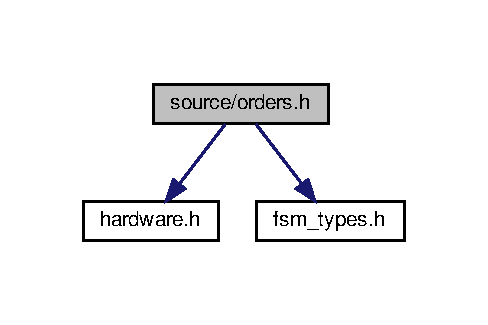
\includegraphics[width=234pt]{orders_8h__incl}
\end{center}
\end{figure}
This graph shows which files directly or indirectly include this file\+:
\nopagebreak
\begin{figure}[H]
\begin{center}
\leavevmode
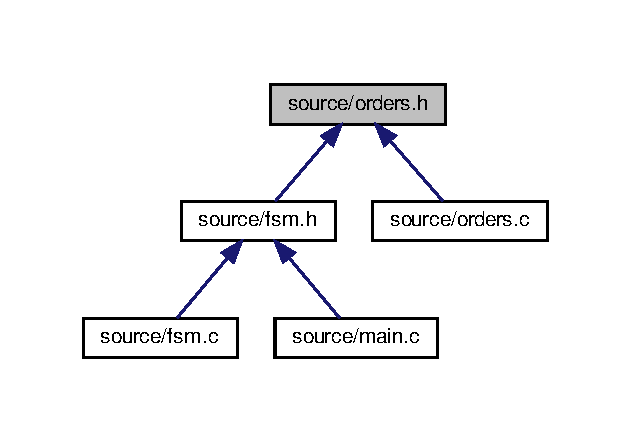
\includegraphics[width=303pt]{orders_8h__dep__incl}
\end{center}
\end{figure}
\subsection*{Functions}
\begin{DoxyCompactItemize}
\item 
\mbox{\Hypertarget{orders_8h_a3ff9b8bfbe60a73d4d0980b7806a4b18}\label{orders_8h_a3ff9b8bfbe60a73d4d0980b7806a4b18}} 
void \hyperlink{orders_8h_a3ff9b8bfbe60a73d4d0980b7806a4b18}{orders\+\_\+clear\+\_\+orders} ()
\begin{DoxyCompactList}\small\item\em Clear {\ttfamily orders\+\_\+matrix}. \end{DoxyCompactList}\item 
int \hyperlink{orders_8h_a36f90d5696f3d3794ab5f07c695c9f17}{orders\+\_\+empty} ()
\begin{DoxyCompactList}\small\item\em Check if {\ttfamily orders\+\_\+matrix} is empty. \end{DoxyCompactList}\item 
void \hyperlink{orders_8h_a3622c7b27d1d98a2ea2de802848f8f44}{orders\+\_\+delete\+\_\+order} (int floor, \hyperlink{hardware_8h_a796a8de8ce0ae769d7dbd3327a7bdbe7}{Hardware\+Order} order\+\_\+type)
\begin{DoxyCompactList}\small\item\em Delete order at {\ttfamily floor} of type {\ttfamily order\+\_\+type} from {\ttfamily orders\+\_\+matrix}. \end{DoxyCompactList}\item 
void \hyperlink{orders_8h_a516839aed0f9113e0546029656518c38}{orders\+\_\+add\+\_\+order} (int floor, \hyperlink{hardware_8h_a796a8de8ce0ae769d7dbd3327a7bdbe7}{Hardware\+Order} order\+\_\+type)
\begin{DoxyCompactList}\small\item\em Add order at {\ttfamily floor} of type {\ttfamily order\+\_\+type} to {\ttfamily orders\+\_\+matrix}. \end{DoxyCompactList}\item 
int \hyperlink{orders_8h_abfb2fa24c83cc212ad124989596a1f58}{orders\+\_\+to\+\_\+handle} (int floor, \hyperlink{fsm__types_8h_a5b298403c88d636ded80069711480dae}{F\+S\+M\+Direction} $\ast$p\+\_\+current\+\_\+direction)
\begin{DoxyCompactList}\small\item\em Check {\ttfamily orders\+\_\+matrix} for orders at {\ttfamily floor} matching the direction of the elevator. \end{DoxyCompactList}\item 
void \hyperlink{orders_8h_a0e3020de74d6e16703fe1348a57e1f78}{orders\+\_\+handled} (int floor)
\begin{DoxyCompactList}\small\item\em Delete all orders at {\ttfamily floor} from {\ttfamily orders\+\_\+matrix}. \end{DoxyCompactList}\item 
void \hyperlink{orders_8h_a3c37f00e1a30d56aa9a42f7e25d34699}{orders\+\_\+get\+\_\+direction} (int floor, \hyperlink{fsm__types_8h_a5b298403c88d636ded80069711480dae}{F\+S\+M\+Direction} $\ast$p\+\_\+current\+\_\+direction)
\begin{DoxyCompactList}\small\item\em Change direction of elevator if there are no matching orders in {\ttfamily orders\+\_\+matrix}. \end{DoxyCompactList}\end{DoxyCompactItemize}


\subsection{Detailed Description}
Functions to collect, prioritize and delete orders. 



\subsection{Function Documentation}
\mbox{\Hypertarget{orders_8h_a516839aed0f9113e0546029656518c38}\label{orders_8h_a516839aed0f9113e0546029656518c38}} 
\index{orders.\+h@{orders.\+h}!orders\+\_\+add\+\_\+order@{orders\+\_\+add\+\_\+order}}
\index{orders\+\_\+add\+\_\+order@{orders\+\_\+add\+\_\+order}!orders.\+h@{orders.\+h}}
\subsubsection{\texorpdfstring{orders\+\_\+add\+\_\+order()}{orders\_add\_order()}}
{\footnotesize\ttfamily void orders\+\_\+add\+\_\+order (\begin{DoxyParamCaption}\item[{int}]{floor,  }\item[{\hyperlink{hardware_8h_a796a8de8ce0ae769d7dbd3327a7bdbe7}{Hardware\+Order}}]{order\+\_\+type }\end{DoxyParamCaption})}



Add order at {\ttfamily floor} of type {\ttfamily order\+\_\+type} to {\ttfamily orders\+\_\+matrix}. 


\begin{DoxyParams}[1]{Parameters}
\mbox{\tt in}  & {\em floor} & \\
\hline
\mbox{\tt in}  & {\em order\+\_\+type} & \\
\hline
\end{DoxyParams}


Definition at line 52 of file orders.\+c.

\mbox{\Hypertarget{orders_8h_a3622c7b27d1d98a2ea2de802848f8f44}\label{orders_8h_a3622c7b27d1d98a2ea2de802848f8f44}} 
\index{orders.\+h@{orders.\+h}!orders\+\_\+delete\+\_\+order@{orders\+\_\+delete\+\_\+order}}
\index{orders\+\_\+delete\+\_\+order@{orders\+\_\+delete\+\_\+order}!orders.\+h@{orders.\+h}}
\subsubsection{\texorpdfstring{orders\+\_\+delete\+\_\+order()}{orders\_delete\_order()}}
{\footnotesize\ttfamily void orders\+\_\+delete\+\_\+order (\begin{DoxyParamCaption}\item[{int}]{floor,  }\item[{\hyperlink{hardware_8h_a796a8de8ce0ae769d7dbd3327a7bdbe7}{Hardware\+Order}}]{order\+\_\+type }\end{DoxyParamCaption})}



Delete order at {\ttfamily floor} of type {\ttfamily order\+\_\+type} from {\ttfamily orders\+\_\+matrix}. 


\begin{DoxyParams}[1]{Parameters}
\mbox{\tt in}  & {\em floor} & \\
\hline
\mbox{\tt in}  & {\em order\+\_\+type} & \\
\hline
\end{DoxyParams}


Definition at line 48 of file orders.\+c.

\mbox{\Hypertarget{orders_8h_a36f90d5696f3d3794ab5f07c695c9f17}\label{orders_8h_a36f90d5696f3d3794ab5f07c695c9f17}} 
\index{orders.\+h@{orders.\+h}!orders\+\_\+empty@{orders\+\_\+empty}}
\index{orders\+\_\+empty@{orders\+\_\+empty}!orders.\+h@{orders.\+h}}
\subsubsection{\texorpdfstring{orders\+\_\+empty()}{orders\_empty()}}
{\footnotesize\ttfamily int orders\+\_\+empty (\begin{DoxyParamCaption}{ }\end{DoxyParamCaption})}



Check if {\ttfamily orders\+\_\+matrix} is empty. 

\begin{DoxyReturn}{Returns}
1 if the order matrix is empty; 0 if it is not. 
\end{DoxyReturn}


Definition at line 37 of file orders.\+c.

\mbox{\Hypertarget{orders_8h_a3c37f00e1a30d56aa9a42f7e25d34699}\label{orders_8h_a3c37f00e1a30d56aa9a42f7e25d34699}} 
\index{orders.\+h@{orders.\+h}!orders\+\_\+get\+\_\+direction@{orders\+\_\+get\+\_\+direction}}
\index{orders\+\_\+get\+\_\+direction@{orders\+\_\+get\+\_\+direction}!orders.\+h@{orders.\+h}}
\subsubsection{\texorpdfstring{orders\+\_\+get\+\_\+direction()}{orders\_get\_direction()}}
{\footnotesize\ttfamily void orders\+\_\+get\+\_\+direction (\begin{DoxyParamCaption}\item[{int}]{floor,  }\item[{\hyperlink{fsm__types_8h_a5b298403c88d636ded80069711480dae}{F\+S\+M\+Direction} $\ast$}]{p\+\_\+current\+\_\+direction }\end{DoxyParamCaption})}



Change direction of elevator if there are no matching orders in {\ttfamily orders\+\_\+matrix}. 

Matching orders are orders above if current direction is up; orders below if current direction is down.


\begin{DoxyParams}[1]{Parameters}
\mbox{\tt in}  & {\em floor} & Current floor of the elevator \\
\hline
\mbox{\tt in,out}  & {\em p\+\_\+current\+\_\+direction} & Current direction of the elevator \\
\hline
\end{DoxyParams}


Definition at line 89 of file orders.\+c.

\mbox{\Hypertarget{orders_8h_a0e3020de74d6e16703fe1348a57e1f78}\label{orders_8h_a0e3020de74d6e16703fe1348a57e1f78}} 
\index{orders.\+h@{orders.\+h}!orders\+\_\+handled@{orders\+\_\+handled}}
\index{orders\+\_\+handled@{orders\+\_\+handled}!orders.\+h@{orders.\+h}}
\subsubsection{\texorpdfstring{orders\+\_\+handled()}{orders\_handled()}}
{\footnotesize\ttfamily void orders\+\_\+handled (\begin{DoxyParamCaption}\item[{int}]{floor }\end{DoxyParamCaption})}



Delete all orders at {\ttfamily floor} from {\ttfamily orders\+\_\+matrix}. 


\begin{DoxyParams}[1]{Parameters}
\mbox{\tt in}  & {\em floor} & \\
\hline
\end{DoxyParams}


Definition at line 83 of file orders.\+c.

\mbox{\Hypertarget{orders_8h_abfb2fa24c83cc212ad124989596a1f58}\label{orders_8h_abfb2fa24c83cc212ad124989596a1f58}} 
\index{orders.\+h@{orders.\+h}!orders\+\_\+to\+\_\+handle@{orders\+\_\+to\+\_\+handle}}
\index{orders\+\_\+to\+\_\+handle@{orders\+\_\+to\+\_\+handle}!orders.\+h@{orders.\+h}}
\subsubsection{\texorpdfstring{orders\+\_\+to\+\_\+handle()}{orders\_to\_handle()}}
{\footnotesize\ttfamily int orders\+\_\+to\+\_\+handle (\begin{DoxyParamCaption}\item[{int}]{floor,  }\item[{\hyperlink{fsm__types_8h_a5b298403c88d636ded80069711480dae}{F\+S\+M\+Direction} $\ast$}]{p\+\_\+current\+\_\+direction }\end{DoxyParamCaption})}



Check {\ttfamily orders\+\_\+matrix} for orders at {\ttfamily floor} matching the direction of the elevator. 

Matching orders are cab orders, orders of same direction or, if no matching orders at other floors, orders of opposite direction.


\begin{DoxyParams}[1]{Parameters}
\mbox{\tt in}  & {\em floor} & Current floor of the elevator \\
\hline
\mbox{\tt in}  & {\em p\+\_\+current\+\_\+direction} & Current direction of the elevator\\
\hline
\end{DoxyParams}
\begin{DoxyReturn}{Returns}
1 if there are matching orders; 0 if there are none. 
\end{DoxyReturn}


Definition at line 57 of file orders.\+c.


\hypertarget{timer_8h}{}\section{source/timer.h File Reference}
\label{timer_8h}\index{source/timer.\+h@{source/timer.\+h}}


Functions to stop and start timer, and detect a timeout.  


{\ttfamily \#include $<$sys/time.\+h$>$}\newline
Include dependency graph for timer.\+h\+:\nopagebreak
\begin{figure}[H]
\begin{center}
\leavevmode
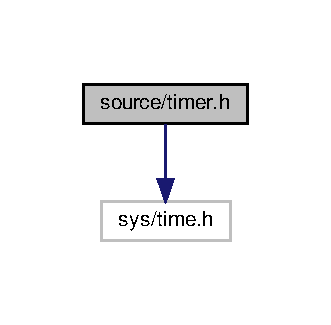
\includegraphics[width=159pt]{timer_8h__incl}
\end{center}
\end{figure}
This graph shows which files directly or indirectly include this file\+:\nopagebreak
\begin{figure}[H]
\begin{center}
\leavevmode
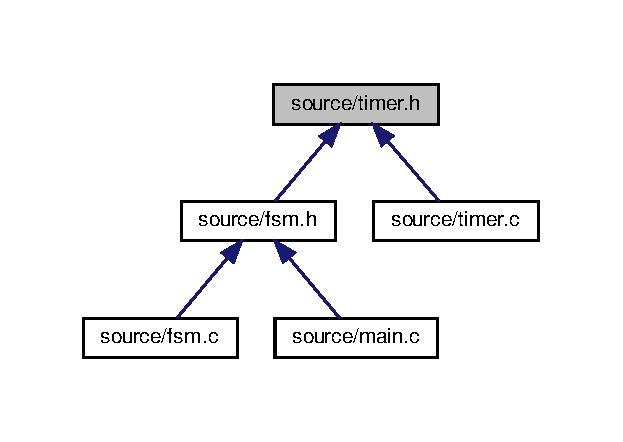
\includegraphics[width=299pt]{timer_8h__dep__incl}
\end{center}
\end{figure}
\subsection*{Functions}
\begin{DoxyCompactItemize}
\item 
void \hyperlink{timer_8h_a338afde680a352415f6f5dd9f5527bac}{timer\+\_\+start} (double duration)
\begin{DoxyCompactList}\small\item\em Start timer with a given {\ttfamily duration}. \end{DoxyCompactList}\item 
void \hyperlink{timer_8h_aa04078f48a0e8f5b6860a393ad06b535}{timer\+\_\+stop} ()
\begin{DoxyCompactList}\small\item\em Stop timer. \end{DoxyCompactList}\item 
int \hyperlink{timer_8h_abde180f78ad23d38b97ce61231320ab2}{timer\+\_\+timeout} ()
\begin{DoxyCompactList}\small\item\em Check if timer has timed out. \end{DoxyCompactList}\end{DoxyCompactItemize}


\subsection{Detailed Description}
Functions to stop and start timer, and detect a timeout. 



\subsection{Function Documentation}
\mbox{\Hypertarget{timer_8h_a338afde680a352415f6f5dd9f5527bac}\label{timer_8h_a338afde680a352415f6f5dd9f5527bac}} 
\index{timer.\+h@{timer.\+h}!timer\+\_\+start@{timer\+\_\+start}}
\index{timer\+\_\+start@{timer\+\_\+start}!timer.\+h@{timer.\+h}}
\subsubsection{\texorpdfstring{timer\+\_\+start()}{timer\_start()}}
{\footnotesize\ttfamily void timer\+\_\+start (\begin{DoxyParamCaption}\item[{double}]{duration }\end{DoxyParamCaption})}



Start timer with a given {\ttfamily duration}. 


\begin{DoxyParams}[1]{Parameters}
\mbox{\tt in}  & {\em duration} & \\
\hline
\end{DoxyParams}


Definition at line 13 of file timer.\+c.

\mbox{\Hypertarget{timer_8h_aa04078f48a0e8f5b6860a393ad06b535}\label{timer_8h_aa04078f48a0e8f5b6860a393ad06b535}} 
\index{timer.\+h@{timer.\+h}!timer\+\_\+stop@{timer\+\_\+stop}}
\index{timer\+\_\+stop@{timer\+\_\+stop}!timer.\+h@{timer.\+h}}
\subsubsection{\texorpdfstring{timer\+\_\+stop()}{timer\_stop()}}
{\footnotesize\ttfamily void timer\+\_\+stop (\begin{DoxyParamCaption}{ }\end{DoxyParamCaption})}



Stop timer. 

Make timer inactive. 

Definition at line 18 of file timer.\+c.

\mbox{\Hypertarget{timer_8h_abde180f78ad23d38b97ce61231320ab2}\label{timer_8h_abde180f78ad23d38b97ce61231320ab2}} 
\index{timer.\+h@{timer.\+h}!timer\+\_\+timeout@{timer\+\_\+timeout}}
\index{timer\+\_\+timeout@{timer\+\_\+timeout}!timer.\+h@{timer.\+h}}
\subsubsection{\texorpdfstring{timer\+\_\+timeout()}{timer\_timeout()}}
{\footnotesize\ttfamily int timer\+\_\+timeout (\begin{DoxyParamCaption}{ }\end{DoxyParamCaption})}



Check if timer has timed out. 

Check if the duration has passed and the timer is active.

\begin{DoxyReturn}{Returns}
1 if the timer has timed out; 0 if not. 
\end{DoxyReturn}


Definition at line 22 of file timer.\+c.


%--- End generated contents ---

% Index
\backmatter
\newpage
\phantomsection
\clearemptydoublepage
\addcontentsline{toc}{chapter}{Index}
\printindex

\end{document}
